\documentclass[12pt,a4paper]{article}

\usepackage[utf8]{inputenc}
\usepackage[T1]{fontenc}
\usepackage{graphicx}
\usepackage{geometry}
\geometry{margin=1in}
\usepackage{hyperref}
\usepackage{enumitem}
\usepackage{caption}
\usepackage{float}
\usepackage{xcolor}
\usepackage{fancyhdr}
\usepackage{titlesec}
\usepackage{amsmath, amssymb}
\usepackage{array}
\usepackage{parskip}
\usepackage{booktabs}
\usepackage{longtable}
\usepackage{xurl}
\usepackage{tikz}
\usetikzlibrary{arrows.meta, positioning, shapes.multipart, shapes.geometric, calc, fit, backgrounds}
\usepackage{listings}

\urlstyle{tt}
\newcommand{\code}[1]{\texttt{\url{#1}}}
% \cls: monospaced identifier that can wrap inside narrow table cells (fixes overlapping text)
\newcommand{\cls}[1]{\nolinkurl{#1}}

% ---- Team members (edit once, used everywhere) ----
\newcommand{\ma}{Ahmad Nawaz}
\newcommand{\mb}{Anamta Akmal}
\newcommand{\mc}{Jagtar Singh}

\newcolumntype{L}[1]{>{\raggedright\arraybackslash}p{#1}}

\lstset{
  basicstyle=\ttfamily\footnotesize,
  breaklines=true,
  frame=single,
  backgroundcolor=\color{gray!8},
  columns=fullflexible,
  keepspaces=true
}

\hypersetup{
    colorlinks=true,
    linkcolor=blue,
    filecolor=magenta,
    urlcolor=cyan,
    citecolor=blue
}

\setlength{\emergencystretch}{3em}

\pagestyle{fancy}
\fancyhf{}
\rhead{SE423 - Milestone 2}
\lhead{Mini API Gateway (MAG)}
\rfoot{Page \thepage}
\setlength{\headheight}{14.5pt}

\titleformat{\section}
 {\normalfont\Large\bfseries\color{black}}{\thesection}{1em}{}
\titleformat{\subsection}
 {\normalfont\large\bfseries\color{black}}{\thesubsection}{1em}{}
\titleformat{\subsubsection}
 {\normalfont\normalsize\bfseries\color{black}}{\thesubsubsection}{1em}{}

\setlength{\parskip}{0.7em}
\setlength{\parindent}{0pt}
\renewcommand{\arraystretch}{1.25}

% ---- UML diagram styles and helpers ----
\newcommand{\st}[1]{\guillemotleft#1\guillemotright}      % stereotype «...»
\newcommand{\cn}[1]{{\centering #1\par}}   % centred class-name compartment

\tikzset{
  % arrows
  assoc/.style={-{Straight Barb[length=5pt,width=6pt]}, line width=0.6pt},      % directed association (open arrow)
  dep/.style={dashed, -{Straight Barb[length=5pt,width=6pt]}, line width=0.6pt},% dependency (dashed, open arrow)
  realize/.style={dashed, -{Triangle[open,length=8pt,width=8pt]}, line width=0.6pt}, % realization
  pl/.style={dashed, line width=0.6pt},                                          % realization feeder line
  call/.style={-{Stealth[length=5pt,width=6pt]}, line width=0.8pt},              % external call
  lbl/.style={font=\tiny, inner sep=1pt, fill=white},
  role/.style={font=\tiny, inner sep=1.5pt, align=left},
  % class box: name | attributes | operations
  class/.style={draw, rectangle split, rectangle split parts=3,
    rectangle split part fill={gray!12,white,white},
    font=\scriptsize, align=left, text width=4.6cm, inner xsep=4pt, inner ysep=3pt},
  note/.style={draw, dashed, font=\tiny, align=left, inner sep=3pt, fill=yellow!10},
  % component diagram
  comp/.style={draw, fill=white, minimum width=3.8cm, minimum height=0.9cm,
    align=center, font=\small, inner xsep=14pt},
  boundary/.style={draw, rounded corners=2pt, fill=gray!5, thick}
}

% component icon (rectangle with two small rectangles on the left edge), top-right corner
\newcommand{\compicon}[1]{%
  \begin{scope}[shift={($(#1.north east)+(-0.32,-0.12)$)}, line width=0.3pt]
    \draw[fill=white] (0,0) rectangle (0.24,-0.16);
    \draw[fill=white] (-0.06,-0.03) rectangle (0.04,-0.07);
    \draw[fill=white] (-0.06,-0.09) rectangle (0.04,-0.13);
  \end{scope}}



% M2 evidence placeholders should be replaced only with verified facts.
\newcommand{\todo}[1]{\textcolor{red!70!black}{\textbf{[TO COMPLETE: #1]}}}
\newcommand{\evidence}[1]{\texttt{#1}}

\begin{document}
\begin{titlepage}
\centering
\IfFileExists{Giki Logo.png}{\includegraphics[width=0.4\textwidth]{Giki Logo.png}}{\vspace*{1cm}}
\vspace{1cm}
{\Huge\bfseries Mini API Gateway (MAG): A Lightweight, Resilient Reverse Proxy\par}
\vspace{1cm}
{\LARGE Joint Semester Project -- Milestone 2\\Working Architecture, Patterns, Concurrency \& Verification Baseline\par}
\vspace{1cm}
{\Large\bfseries SE423: Software Construction and Development\par}
\vspace{0.5cm}
{\large Instructor: Dr. Mian Muaz Razaq\par}
\vspace{0.6cm}
{\large\bfseries Submitted By:\par}
\vspace{0.3cm}
\begin{tabular}{ll}\ma & 2023085 \\\mb & 2023113 \\\mc & 2023266\end{tabular}
\vspace{0.7cm}
{\large Repository: \url{https://github.com/jagtar5/MiniApiGateway}\par}
\vspace{\fill}
\textit{Faculty of Computer Science and Engineering}\\
\textit{GIK Institute of Engineering Sciences and Technology}\\[0.4cm]
{\large Date: \todo{submission date}\par}
\end{titlepage}
\tableofcontents
\newpage

\section{Introduction and Milestone 2 Rubric Coverage}
This report documents the \emph{implemented} Milestone~2 build of the Mini API Gateway (MAG). It follows the Milestone~1 design and references only code, tests and artifacts verified at the submitted commit. Any incomplete implementation is identified as such rather than represented as complete.
\begin{table}[H]\centering\small
\begin{tabular}{L{6cm} c L{5.2cm}}\toprule
\textbf{SE423 M2 criterion} & \textbf{Weight} & \textbf{Evidence in this report}\\\midrule
Working core architecture & 20\% & Section~\ref{sec:core}\\
Design patterns implemented correctly & 20\% & Section~\ref{sec:patterns}\\
Defensive programming and exception handling & 10\% & Section~\ref{sec:defensive}\\
Concurrency and thread-safety implementation & 15\% & Section~\ref{sec:concurrency}\\
Code quality and SOLID adherence & 15\% & Section~\ref{sec:solid}\\
TDD and automated-test baseline & 10\% & Section~\ref{sec:tdd}\\
Repository discipline and traceability & 10\% & Section~\ref{sec:repo}\\\bottomrule
\end{tabular}\caption{SE423 M2 rubric cross-reference.}\end{table}
\textbf{Submitted source revision:} integrated branch \texttt{feature/js-integration} at commit \texttt{2780b4c9da3db887c89ebe58c392c61bc99ae3e6}; \texttt{m2-baseline} is not present and is not claimed as evidence.

\section{Working Core Architecture (20\%)}\label{sec:core}
\subsection{Architecture Compared with Milestone 1}
The proposed system consists of \textbf{M-A} Proxy Pipeline, \textbf{M-B} Identity \& Traffic Control, \textbf{M-C} Fast-Path Cache, \textbf{M-D} Resilience Engine and \textbf{M-E} Configuration \& Admin. The Maven modules are \texttt{gateway-core} and \texttt{gateway-app}; the former contains domain logic and the latter the Spring Boot application shell.
\begin{longtable}{L{1.2cm} L{3.8cm} L{2cm} L{5.2cm}}\toprule
\textbf{Module} & \textbf{M2 functionality} & \textbf{Status} & \textbf{Code/test evidence}\\\midrule\endhead
M-A & Request ID, JWT authentication, forwarding, exception mapping & \todo{status} & \todo{classes and test links}\\
M-B & Token bucket, fixed and sliding window, rate-limit filter & \todo{status} & \todo{classes and test links}\\
M-C & GET/200 bounded cache, TTL, single-flight & Implemented & \evidence{CachingUpstreamClient}, \evidence{BoundedLruCache}; 12 cache tests plus 100-request stampede test\\
M-D & Circuit breaker closed/open/half-open lifecycle & Implemented & \evidence{CircuitBreaker}, \evidence{ClosedState}, \evidence{OpenState}, \evidence{HalfOpenState}; 8 breaker/resilience tests\\
M-E & Persistence, admin API, validation, snapshot reload & \todo{status} & \todo{classes and test links}\\\bottomrule\end{longtable}
\subsection{Request Path and Integration}
Planned filter order: \texttt{RequestIdFilter} $\rightarrow$ \texttt{AuthFilter} $\rightarrow$ \texttt{RateLimitFilter} $\rightarrow$ \texttt{ForwardFilter}. Planned upstream decorator order: \texttt{CachingUpstreamClient} $\rightarrow$ \texttt{ResilientUpstreamClient} $\rightarrow$ \texttt{HttpUpstreamClient}. \todo{confirm actual order against merged code}.
\begin{figure}[H]\centering
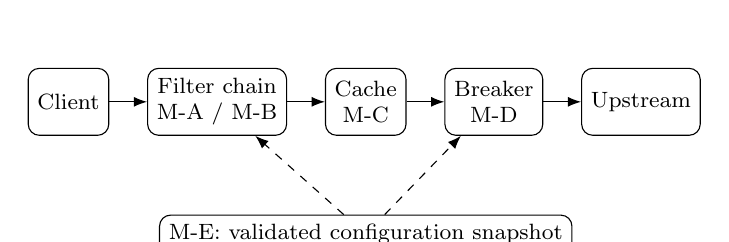
\begin{tikzpicture}[node distance=0.55cm and 0.48cm, every node/.style={font=\footnotesize}, >=Latex]
\node[draw,rounded corners,minimum height=0.85cm] (client) {Client};
\node[draw,rounded corners,right=of client,minimum height=0.85cm,align=center] (filters) {Filter chain\\M-A / M-B};
\node[draw,rounded corners,right=of filters,minimum height=0.85cm,align=center] (cache) {Cache\\M-C};
\node[draw,rounded corners,right=of cache,minimum height=0.85cm,align=center] (breaker) {Breaker\\M-D};
\node[draw,rounded corners,right=of breaker,minimum height=0.85cm,align=center] (up) {Upstream};
\draw[->] (client)--(filters);\draw[->](filters)--(cache);\draw[->](cache)--(breaker);\draw[->](breaker)--(up);
\node[draw,rounded corners,below=1cm of cache,align=center] (config) {M-E: validated configuration snapshot};
\draw[->,dashed] (config)--(filters);\draw[->,dashed] (config)--(breaker);
\end{tikzpicture}
\caption{Proposed integration view; revise if actual wiring differs.}\end{figure}
\subsection{End-to-End Demonstration}
\begin{longtable}{L{4.3cm} L{4.2cm} L{4.1cm}}\toprule
\textbf{Scenario} & \textbf{Expected} & \textbf{Observed result / evidence}\\\midrule\endhead
Valid signed JWT to \texttt{/fast} & Proxied upstream response & \todo{HTTP result and run link}\\
Missing/invalid JWT & HTTP 401; no upstream call & \todo{result}\\
Rate limit $N+1$ & HTTP 429 and Retry-After & \todo{result}\\
Flaky upstream circuit threshold & Breaker opens and fails fast & \todo{result}\\
Cacheable repeated GET & Second request served from safe cache & \todo{result}\\
Invalid configuration reload & Previous snapshot remains active & \todo{result}\\\bottomrule\end{longtable}
\subsection{Milestone 2 M-C Cache Implementation (Jagtar Singh)}
Source evidence: \evidence{gateway-core/src/main/java/com/mag/core/upstream/impl/CachingUpstreamClient.java}, \evidence{.../cache/BoundedLruCache.java} and \evidence{.../cache/CacheKey.java}. \texttt{CachingUpstreamClient} is a structural Proxy implementation of \texttt{UpstreamClient}. It bypasses caching for non-GET requests, derives a per-user/request cache key through \texttt{CacheKey}, returns only unexpired GET/200 responses, and delegates misses to \texttt{executeSingleFlight}. The backing \texttt{BoundedLruCache} is an access-order \texttt{LinkedHashMap} guarded by a \texttt{ReentrantLock}; setting \texttt{removeEldestEntry} to enforce the configured maximum provides bounded LRU eviction. TTL is injected through \texttt{Clock}: a response Cache-Control \texttt{max-age} overrides the configured default, and the local M-C fix falls back to the default when an oversized or malformed numeric value would overflow parsing.

Cache eligibility is explicit: only GET and HTTP 200 responses are considered, while Set-Cookie, private and no-store responses are excluded. \texttt{CacheKey} includes authenticated identity information so separate users do not share profile/cache entries. Single-flight loading uses a \texttt{ConcurrentHashMap<CacheKey, CompletableFuture<UpstreamResponse>>}; the first requester owns the upstream call and competing callers join the same future. This implementation is proved by tests in \texttt{CachingUpstreamClientTest.java}, including cache hit/miss, TTL, LRU eviction, 100 concurrent misses, user separation, non-GET/non-200 and private/Set-Cookie exclusions.

\subsection{Milestone 2 M-D Circuit Breaker Implementation (Jagtar Singh)}
Source evidence: \evidence{gateway-core/src/main/java/com/mag/core/resilience/CircuitBreaker.java} and \evidence{gateway-core/src/main/java/com/mag/core/resilience/impl/}. \texttt{CircuitBreaker} uses the State pattern. \texttt{ClosedState} is the initial state and permits requests; \texttt{OpenState} fails fast until the open timeout has elapsed; then it CAS-transitions to \texttt{HalfOpenState}, whose probe allowance is tracked with atomic counters. A successful required probe set transitions back to CLOSED, while a probe failure immediately opens the circuit again. \texttt{AtomicReference<CircuitState>} and \texttt{transitionTo(...)} provide atomic state replacement by compare-and-set. Failure counting in CLOSED uses \texttt{AtomicInteger} and a clock-controlled failure window.

The actual proof is \texttt{CircuitBreakerTest.java}: 8 breaker tests cover initial CLOSED, threshold-to-OPEN, OPEN timeout, HALF-OPEN recovery, HALF-OPEN re-open, probe limits, success reset and 20-thread concurrent failures. The gateway integration test also verifies that an OPEN breaker maps to HTTP 503. \texttt{ResilientUpstreamClient} reports 5xx and exceptions to the breaker, and a null response is mapped locally to HTTP 502/\texttt{UpstreamUnavailableException} after the M-D defensive fix.

\subsection{Milestone 2 Dashboard Integration (Jagtar Singh)}
Source evidence: \evidence{gateway-app/src/main/resources/static/index.html}, \evidence{gateway-app/src/main/resources/static/dashboard.js} and \evidence{gateway-app/src/test/java/com/mag/app/GatewayIntegrationTest.java}. The implemented static dashboard consists of the three panels shown in \texttt{index.html}: Live Metrics, Routes \& Active Rules, and Gateway Request Tester. \texttt{dashboard.js} calls \texttt{/admin/metrics}, \texttt{/admin/routes} and \texttt{/api/**}. The metrics panel displays allowed, blocked, cache-hit ratio and circuit state. The routes panel lists route data and supports authenticated TTL updates. The tester dispatches the selected method/path through the gateway and shows the response. Credentials are entered in the page and are sent as Authorization headers; they are not stored in source or persisted. \texttt{GatewayIntegrationTest.testDashboardStaticFiles}, \texttt{testAdminMetricsSecurity}, \texttt{testAdminRoutesListingAndUpdating} and \texttt{testCircuitBreakerFailsFastInGateway} provide integration evidence for the dashboard shell and APIs.

\textbf{Architecture deviations from M1:} The implemented upstream integration remains decorator based: \texttt{CachingUpstreamClient} wraps \texttt{ResilientUpstreamClient}, which wraps the concrete HTTP client. This preserves the M1 proposal. The M-C and M-D implementations are present and tested in \texttt{gateway-core}; database-backed M-E configuration remains an application-shell integration and is not attributed to M-C/M-D.

\section{Implemented Design Patterns (20\%)}\label{sec:patterns}
Document only patterns present and actually connected to the running system. The M1 pattern plan included Chain of Responsibility, Strategy, Factory, State, Proxy and Builder.
\begin{longtable}{L{2.9cm} L{3.3cm} L{3.8cm} L{3.1cm}}\toprule
\textbf{Pattern / type} & \textbf{Concrete classes} & \textbf{Problem and benefit} & \textbf{Code/test proof}\\\midrule\endhead
Chain of Responsibility (behavioral) & GatewayFilter, FilterChain & Ordered independent request processing & \todo{evidence}\\
Strategy (behavioral) & RateLimitAlgorithm implementations & Replace limits without rewriting filter & \todo{evidence}\\
Factory (creational) & RateLimiterFactory & Register and construct algorithms & \todo{evidence}\\
State (behavioral) & \evidence{CircuitState}, \evidence{ClosedState}, \evidence{OpenState}, \evidence{HalfOpenState} & Explicit closed/open/half-open transitions and fail-fast behavior & \evidence{CircuitBreakerTest.java}: initial, threshold, open timeout, half-open recovery, probe limit and concurrent failures\\
Proxy (structural) & \evidence{CachingUpstreamClient}, \evidence{ResilientUpstreamClient} & Decorate upstream loading and resilience without changing \evidence{UpstreamClient} & \evidence{CachingUpstreamClientTest.java}: 12 cache tests; cache-hit bypass proof\\
Builder (creational) & PipelineBuilder & Safe assembly of ordered filters & \todo{evidence}\\\bottomrule\end{longtable}
\textbf{Rejected alternatives and rationale:} For M-D, a boolean flag and one large \texttt{if/else} would have concentrated state transitions in \texttt{CircuitBreaker}, making open, probe and recovery behavior harder to isolate and test. The State pattern gives each state one transition policy. For M-C, subclassing or duplicating the HTTP client for caching was rejected because it would change multiple upstream implementations and hide cache behavior outside the \texttt{UpstreamClient} contract. The Proxy/decorator approach preserves the existing contract and allows cache hits to bypass resilience decoration.
\textbf{Runtime proof:} State behavior is proved by \texttt{CircuitBreakerTest}; Proxy/cache behavior is proved by \texttt{CachingUpstreamClientTest} and the cache-hit bypass test; dashboard integration is proved by \texttt{GatewayIntegrationTest}. A complete runtime proof for all M1 patterns remains shared-team evidence and is not replaced by these M-C/M-D demonstrations.

\section{Defensive Programming and Exception Handling (10\%)}\label{sec:defensive}
\begin{longtable}{L{3.3cm} L{4.5cm} L{4.5cm}}\toprule
\textbf{Boundary} & \textbf{Validation / failure policy} & \textbf{Implemented evidence}\\\midrule\endhead
JWT authentication & Missing, malformed, expired, bad signature and \texttt{alg=none} rejected & \todo{tests / 401 response}\\
Route/config inputs & Missing URL/path, negative TTL/rules rejected & \todo{validation tests}\\
Admin API & Authentication/authorization, field-level errors & \todo{API tests}\\
Upstream calls & Timeout and null/5xx failures are reported to resilience logic; null upstream response is an HTTP 502 & \texttt{ResilientUpstreamClientTest}; \texttt{testNullUpstreamResponse} and 5xx fail-fast tests are present\\
Cross-module faults & Structured exceptions; no confidential data in logs & \todo{mapper/logger evidence}\\\bottomrule\end{longtable}
\textbf{Exception hierarchy / status mapping:} \todo{add actual exception classes and mapped statuses}.\\
\textbf{Logging and secret-handling:} \todo{describe verified request IDs and token redaction}.

\section{Concurrency and Thread-Safety (15\%)}\label{sec:concurrency}
\begin{longtable}{L{3cm} L{4cm} L{4.3cm} L{1.5cm}}\toprule
\textbf{Component} & \textbf{Hazard} & \textbf{Actual protection / test} & \textbf{Result}\\\midrule\endhead
Rate limiter & Check-then-act allows over-limit requests & Not implemented in the audited M-B filter; test status pending owner evidence & Pending\\
Cache single-flight & Stampede on same key & \texttt{ConcurrentHashMap<CacheKey, CompletableFuture<...>>}; 100 concurrent cache-miss requests & Exactly 1 upstream call\\
Circuit breaker & Duplicate state transitions & \texttt{AtomicReference<CircuitState>} plus CAS in \texttt{transitionTo}; 20-thread concurrent failure test & OPEN after threshold; no assertion proves one transition versus duplicate CAS observations beyond state test\\
Config hot reload & Reader sees inconsistent state & \todo{immutable snapshot and AtomicReference} & \todo{value}\\\bottomrule\end{longtable}
\textbf{Concurrency proof:} M-C used 100 simultaneous cache-miss requests and observed exactly one upstream call. M-D used 20 simultaneous failure reports against threshold 5 and ended in OPEN state. These tests are repository tests, but a green GitHub Actions CI run and shared CI artifact link are not yet present.\\
\textbf{Thread safety document:} \evidence{docs/thread-safety-strategy.md} was not found in the audited repository; it remains a pending M2 evidence item.

\section{Code Quality and SOLID Adherence (15\%)}\label{sec:solid}
\begin{longtable}{L{1cm} L{5.6cm} L{5.7cm}}\toprule
\textbf{SOLID} & \textbf{Applied design decision} & \textbf{Actual code / test proof}\\\midrule\endhead
S & Cache loading and bounded storage are separated into \evidence{CachingUpstreamClient} and \evidence{BoundedLruCache}; circuit delegation and state policy are separated into \evidence{CircuitBreaker} and state classes & Source paths in \texttt{gateway-core/src/main/java/com/mag/core/upstream/impl} and \texttt{.../resilience}\\
O & Extend RateLimitAlgorithm via registry & \todo{dummy strategy extension test}\\
L & Replace UpstreamClient and rate-limit implementations under contract & \todo{parametrized contract tests}\\
I & Small filter, client and configuration interfaces & \todo{interface signatures}\\
D & M-C and M-D depend on the \evidence{UpstreamClient}, \evidence{Clock} and \evidence{CircuitState} abstractions; constructors receive implementations from application composition or tests & \evidence{CachingUpstreamClient}, \evidence{CircuitBreaker}, \evidence{InfrastructureConfig}\\\bottomrule\end{longtable}
\textbf{Findings and resolutions:} M-C and M-D retain constructor-injected dependencies and implement narrow domain interfaces. No repository-wide SOLID departure is attributed to these modules. The local M-C fix prevents oversized TTL parsing from escaping; the M-D fix prevents null upstream responses from bypassing gateway exception handling.

\section{TDD and Automated-Test Baseline (10\%)}\label{sec:tdd}
The M2 rubric requires test execution against implemented business logic, authentic red--green--refactor history and measured coverage. A 60\% threshold is a final minimum, not an M2 percentage threshold.
\begin{longtable}{L{3.5cm} L{3.6cm} L{5.1cm}}\toprule
\textbf{Evidence} & \textbf{Measured/observed} & \textbf{Artifact}\\\midrule\endhead
Maven unit test summary & 30 passed, 0 failures, 0 errors, 0 skipped in gateway-core & \evidence{gateway-core/target/surefire-reports}\\
Core line coverage (JaCoCo) & 57\% instruction, 54.5\% line, 66\% branch coverage in the actual generated report & \evidence{gateway-core/target/site/jacoco/index.html}\\
Pipeline tests & \todo{status} & \todo{JUnit files}\\
Rate-limit/concurrency tests & \todo{status} & \todo{JUnit files}\\
Cache and breaker tests & Core suite: 30 tests run, 0 failures, 0 errors; cache suite 12 tests, breaker/resilience suite 8 or more tests & \evidence{CachingUpstreamClientTest.java}, \evidence{CircuitBreakerTest.java}, \evidence{ResilientUpstreamClientTest.java}\\
Integration tests & Gateway integration test file present; execution status not claimed without a run artifact & \evidence{GatewayIntegrationTest.java}\\
Red/green/refactor trace & Test and implementation commits exist for M-C/M-D; no refactor-only commit or complete team trail was verified & \texttt{9b78180}/\texttt{8094301} and \texttt{a7b6f1c}/\texttt{ef37bd6}\\\bottomrule\end{longtable}
\textbf{Verification command(s):} \texttt{mvn -pl gateway-core test checkstyle:check}; \texttt{mvn -pl gateway-core jacoco:report}. The full integration/\texttt{clean verify} gate was not claimed because it was not run successfully under the audited environment.\\
\textbf{Coverage gaps:} The generated core report measured 57\% instruction, 54.5\% line and 66\% branch coverage. M-C cache and M-C upstream implementation coverage is 88\% and 79\% instruction respectively; resilience implementation packages are approximately 86--87\% instruction. Remaining gaps include the unimplemented M-B filter and other owner-owned modules. A final green CI/coverage gate and integration-module JaCoCo report remain pending.

\section{Repository Discipline and Contribution Traceability (10\%)}\label{sec:repo}
\begin{longtable}{L{3.0cm} L{4.3cm} L{5cm}}\toprule
\textbf{Control} & \textbf{Agreed approach} & \textbf{M2 evidence}\\\midrule\endhead
Branching & Independent feature branches and PRs & Feature branches include \texttt{feature/js-cache}, \texttt{feature/js-resilience} and \texttt{feature/js-integration}; PR \#1 and PR \#2 are merged, while at least one additional PR is still targeted by the plan\\
Review & Non-author reviewer for merges & PR \#1 and PR \#2 are merged, but GitHub returned no reviews or comments; non-author reviewer evidence is pending\\
CI gate & Build and tests on push/PR & No GitHub Actions workflow or run was exposed; this remains a repository blocker, not claimed as passing\\
TDD commit trail & \texttt{test:}, \texttt{feat:}, \texttt{refactor:} commits & JS examples: \texttt{9b78180}, \texttt{8094301}, \texttt{a7b6f1c}, \texttt{ef37bd6}; evidence commit \texttt{7913638} added M2 reports and M-C/M-D fixes\\
Baseline & Annotated \texttt{m2-baseline} tag & No local or remote \texttt{m2-baseline} exists; no tag was created or moved\\
AI transparency & Recorded significant assisted changes & \todo{AI log path/entry IDs}\\\bottomrule\end{longtable}
\subsection{Individual Responsibility and Evidence}
\begin{longtable}{L{2.7cm} L{4.4cm} L{5.2cm}}\toprule
\textbf{Member} & \textbf{Owned work} & \textbf{PR / tests / review evidence}\\\midrule\endhead
\ma & M-A, SOLID tests, CI and construction evidence & \todo{links}\\
\mb & M-B, M-E and concurrency tests & \todo{links}\\
\mc & M-C, M-D, integration and dashboard & Commits \texttt{9b78180}, \texttt{8094301}, \texttt{a7b6f1c}, \texttt{ef37bd6}, \texttt{56cf134}; M2 audit and static-analysis reports; PR \#1 merged without recorded reviewer evidence\\\bottomrule\end{longtable}

\section{M2 Build Reproduction and Handover}
\textbf{Environment:} Verified for local evidence: Apache Maven 3.9.11 and Oracle JDK 24.0.2. SpotBugs could not analyze JDK 24 class files because SpotBugs 4.8.6 reported unsupported major version 68. Docker and a final integration database/JDK 21 verification remain pending.\\
\textbf{Setup and start steps:} \todo{copy verified README commands and environment variables without secrets}.\\
\textbf{Known limitations:} M-B \texttt{RateLimitFilter.doFilter()} remains a stub. Branch protection is reported enabled, so retain authenticated settings evidence. GitHub Actions, JDK 21 SpotBugs rerun, final integration execution, thread-safety strategy document, non-author PR approval and \texttt{m2-baseline} remain high-priority blockers. SpotBugs produced no usable finding set under JDK 24; Checkstyle reported 0 core violations after the M-C/M-D cleanup and 3 app findings deferred outside M-C/M-D.\\
\textbf{M3 follow-ups:} \todo{coverage improvements, refactoring, robustness and final demo actions}.

\section*{Conclusion}
The M-C bounded cache and M-D circuit breaker are implemented and have repository/JUnit evidence. The cache covers hit/miss, TTL, LRU eviction, single-flight, user separation and cache eligibility; the breaker covers closed/open/half-open transitions and concurrent state change. The three-panel dashboard and its integration APIs are implemented and integration tests exist. Repository and M2 governance evidence remain incomplete: CI, branch protection, multiple merged/reviewed PRs and \texttt{m2-baseline} are pending verification.
\end{document}